\documentclass[tikz,border=10pt]{standalone}
\usepackage{tikz}
\usetikzlibrary{calc}

\begin{document}
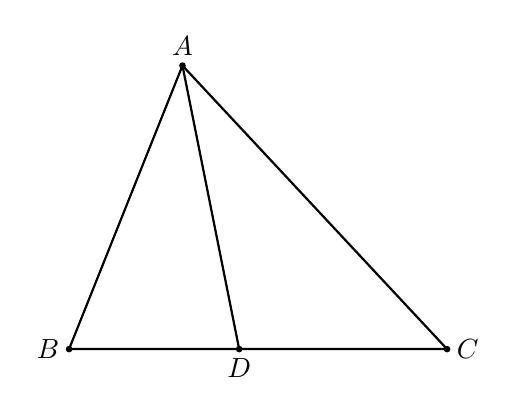
\begin{tikzpicture}[>=stealth, scale=1.2]
    % 1. 定义关键坐标点
    % 这里根据原图视觉比例设置坐标：A为顶点，B/C为底端
    \coordinate (A) at (1.2, 3);
    \coordinate (B) at (0, 0);
    \coordinate (C) at (4, 0);
    % D 点位于线段 BC 上，约在 1/3 处
    \coordinate (D) at (1.8, 0);

    % 2. 绘制三角形轮廓和内部线段
    \draw [thick] (A) -- (B) -- (C) -- cycle; % 绘制三角形 ABC
    \draw [thick] (A) -- (D);                % 绘制线段 AD

    % 3. 绘制顶点处的圆点 (可选，原图中有微小黑点)
    \foreach \p in {A, B, C, D}
        \fill (\p) circle (1pt);

    % 4. 标注字母标签
    % anchor 参数用于调整文字相对于坐标点的方位，以防遮挡线条
    \node [above] at (A) {$A$};
    \node [left]  at (B) {$B$};
    \node [right] at (C) {$C$};
    \node [below] at (D) {$D$};

\end{tikzpicture}
\end{document}